% 03_markovnet.tex
In this section, we consider methods for exploiting temporal correlation between CSI of subsequent timeslots.
Assuming the channel does not change substantially within a certain window of time,
a reasonably accurate CSI estimate at some time $t-1$ can be used to estimate the CSI at time $t$.
Generically, we can write this estimator as
\begin{align}
\hat{\mathbf H}_t &= h(\hat{\mathbf H}_{t-1}) \label{eq:gen_estim}
\end{align}
where $\mathbf{H}_t$ is the CSI matrix at time $t$ and $\hat{\mathbf H}_t$ is its estimator. 
The estimation error under $\hat H_t$ is
\begin{align}
\mathbf E_{t} &= \mathbf H_{t} - \hat{\mathbf H}_{t}. \label{eq:diff_err}
\end{align}

\subsection{Related Work}

Non ML-based work in temporal correlation for CSI estimation utilized state-space methods such as the Kalman filter \cite{ref:Huber2006improved,ref:Ali2020BayesKalmanFilter,ref:Kim2021KalmanVsML}. Since it relies on explicit state space and noise models, the Kalman filter's predictive power in CSI estimation is limited. Furthermore, such work generally does not propose a method for feedback compression, making comparison with the following ML methods difficult.

Recent works have leveraged recurrent neural networks (RNNs) to exploit temporal correlation for CSI estimation \cite{ref:Lu2019RecCsiNet, ref:Liao2019BiLSTM, ref:Li2020SpatTempLSTM,
 ref:Jang2019Delay,ref:Wang2019CsiNetLSTM}. RNNs include recurrent layers, such as the long short-term memory (LSTM) cell or the gated recurrent unit (GRU), which are capable of learning long-term dependencies of a given process through backpropagation \cite{ref:Hermans2013Training} and can be used to predict future states of the process \cite{ref:Pascanu2014HowTo}.

\begin{figure}[htb]
	\centering
	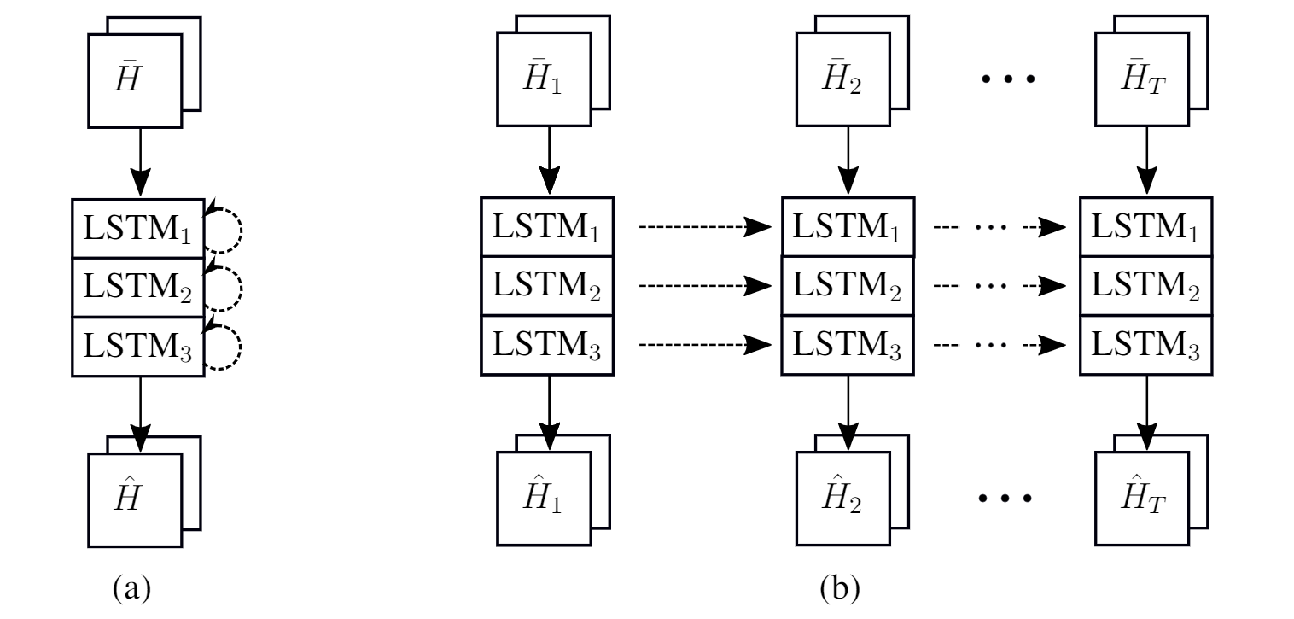
\includegraphics[width=.9\textwidth]{lstm-example-unroll.pdf}
	\medskip
	\caption{An example of LSTMs used for CSI estimation. (a) ``Stacked'' LSTM network of depth 3 shown with recurrent connections. (b) Same LSTM network ``unrolled" into $T$ timeslots }
	\label{fig:lstm_example}
\end{figure}

RNNs have been used extensively in natural language processing (NLP) for machine translation \cite{ref:Sutskever2014seq2seq} and sentiment extraction \cite{ref:Irsoy2014opinion}. For such works in NLP, authors have empirically found ``stacked'' or ``deep'' RNNs to be effective (e.g., Fig.~\ref{fig:lstm_example}), hypothesizing that having multiple recurrent layers allows the network to extract different semantic timescales \cite{ref:Irsoy2014opinion, ref:Bengio2009Learning}. Works in CSI estimation have taken cues from this work in NLP, proposing CSI estimation networks with stacked LSTMs after a sequence of autoencoders \cite{ref:Wang2019CsiNetLSTM}. While such work has demonstrated the utility of RNNs, the computational cost of LSTMs can be prohibitively high. For example, the RNN portion of the network proposed in \cite{ref:Wang2019CsiNetLSTM} accounts for $10^8$ additional parameters. Since channel estimation should not place an undue computational burden on the communications system, LSTMs can be problematic.

\subsection{Methods}

Rather than use RNNs to extract temporal dependencies in CSI data, we proposed a lightweight network based on the principle of differential encoding. We propose to train a network to estimate the error (\ref{eq:diff_err}) when using a simple linear estimator, 
\begin{align*}
\hat{\mathbf H}_t &= \mathbf W \hat{\mathbf H}_{t-1} 
\end{align*}
where $\mathbf W \in \mathbb C^{R_b \times R_b}$ is the minimum mean squared error (MMSE) estimator.
\begin{align*}
\mathbf H_t &= \mathbf W\mathbf H_{t-1} + \mathbf E_t \\
\mathbf H_{t-1}^H\mathbf H_t &= \mathbf W\mathbf H_{t-1}^H\mathbf H_{t-1} + \mathbf H_{t-1}^H\mathbf E_t \\
\end{align*}
Under the principle of orthogonality, the error term $\mathbf E_t$ is orthogonal with the observed data, and the product $\mathbf H^H_{t-1}\mathbf E_t$ becomes a zero matrix. Denoting the cross correlation matrix as $\mathbf R_{i} = \mathbb{E}\left[\mathbf H_{t-i}^H\mathbf H_{t}\right]$.
\begin{align*}
\mathbf W &= \mathbf R_0^{-1} \mathbf R_1 
\end{align*}
We can further simplify this estimator to a scalar, $\gamma \in \mathbb R$, as
\begin{align*}
\gamma &= \frac{\sum_i^{R_d}\sum_j^{N_b}\mathbf R_1(i,j)}{\sum_i^{R_d}\sum_j^{N_b}\mathbf R_0(i,j)},
\end{align*}
where $i$ ($j$) are the row (column) indices of the correlation matrices. Under the estimator $\gamma$, we proposed to encode the error, $\mathbf E_t$, using a convolutional autoencoder, $f(\mathbf E_t)$,
\begin{align*}
\hat{\mathbf E}_t &= g(f(\mathbf E_t, \vec\theta_e), \vec\theta_d),
\end{align*}
where $\mathbf E_t = \mathbf H_t - \gamma\hat{\mathbf H}_{t-1}$. The base station has access to the estimators $\gamma$ and $\hat{\mathbf H}_{t-1}$, and the resulting CSI estimate at $t$ is
\begin{align*}
\hat{\mathbf H}_t &= \gamma \hat{\mathbf H}_{t-1} + \hat{\mathbf{E}}_t
\end{align*}

\subsection{Numerical Results}

We compare MarkovNet with CsiNet-LSTM \cite{ref:Wang2019CsiNetLSTM} on the indoor and outdoor COST2100 datasets (for details, see Section~\ref{sect:channel_model}). For MarkovNet, we train the network at the first timeslot for 1000 epochs. In each subsequent timeslot, we initialize the network using the weights from the previous timeslot and train for 200 epochs. We use a batch size of 200. We perform a training/testing split of 75k/25k samples, and we estimate $\gamma$ using the training set. To compare the estimation accuracy of each network, we report the NMSE.
%estimate of the previous timeslot with the scalar MMSE estimator, $\gamma$, to produce the error term $\mathbf E_t = \mathbf H_t - \gamma\hat{\mathbf H}_{t-1}$.

Figure~\ref{fig:csi_image} shows a random sample from the test set, $\mathbf H$, and the estimates produced by CsiNet-LSTM and MarkovNet for a CR of $\frac 14$. This sample contains three ``peak'' magnitude regions. While both networks manage to capture the two larger samples, MarkovNet is able to recover the small peak magnitude region which CsiNet-LSTM fails to produce.

\begin{figure}[htb] \centering 
	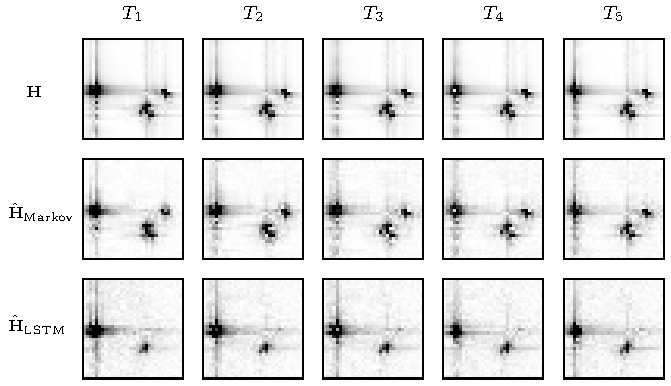
\includegraphics[width=0.9\linewidth]{batch0_csi_compare_cr512.pdf}
	\caption{CSI ($\mathbf H$), MarkovNet estimates ($\hat{\mathbf H}_{\text{Markov}}$), and CsiNet-LSTM estimates ($\hat{\mathbf H}_{\text{LSTM}}$) across five timeslots ($T_1$ through $T_5$) on one outdoor channel sample from the test set,
using $\text{CR}=\frac 14$.} 
	\label{fig:csi_image} 
\end{figure}